% Prof. Dr. Ausberto S. Castro Vera
% UENF - CCT - LCMAT - Curso de Ci\^{e}ncia da Computa\c{c}\~{a}o
% Campos, RJ,  2021
% Disciplina: Paradigmas de Linguagens de Programa\c{c}\~{a}o
%

\chapter{Ferramentas}
Nesse capítulo apresentamos as três principais ferramentas do ecossistema Julia: VScode, Jupyter Notebook e Juno. 
Todos são apresentados com destaque no próprio site da linguagem (Fig \ref{julia_editors_site}), além de ocuparem as primeiras posições no \href{https://julialang.org/blog/2021/08/julia-user-developer-survey/}{questionário anual dos usuários da linguagem} (Fig \ref{julia_editors_survey}).% que coletou respostas de 2 660 em 2021.. 

\begin{figure}[H]
\begin{center}
    \caption{Editores preferidos dos usuários de Julia em 2021} \label{julia_editors_survey}
    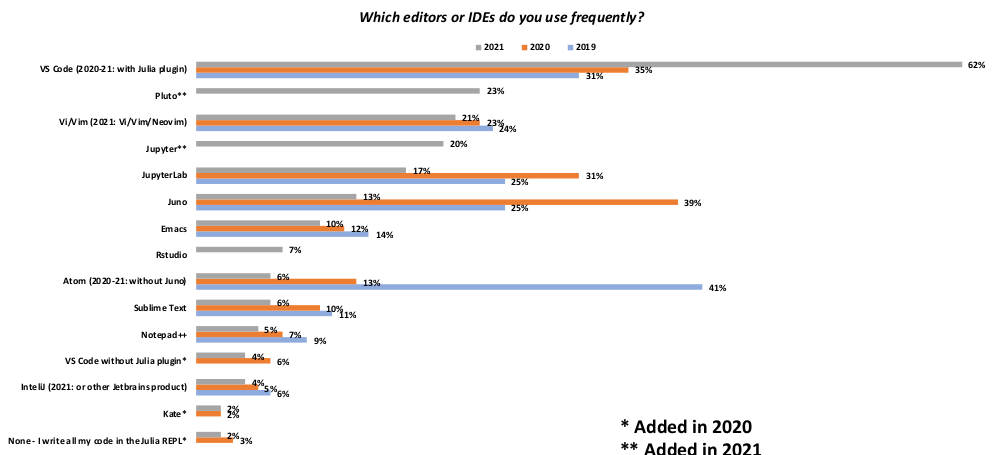
\includegraphics[width=15cm]{aplicacoes/Editores e IDEs.png} \\
    {\tiny \sf Fonte: https://julialang.org/blog/2021/08/julia-user-developer-survey }
\end{center}
\end{figure} 

\begin{figure}[H]
\begin{center}
    \caption{Editores e IDEs destacadas no site da linguagem} \label{julia_editors_site}
    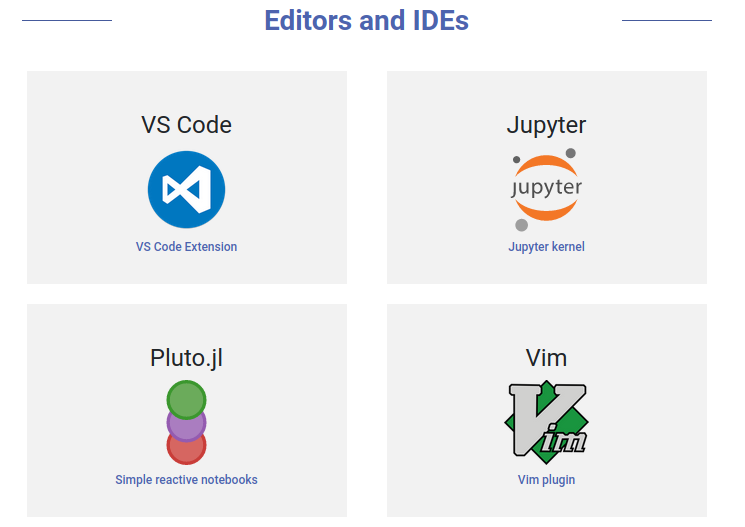
\includegraphics[width=12cm]{aplicacoes/Editors_IDEs_site.png} \\
    {\tiny \sf Fonte: https://julialang.org/}
\end{center}
\end{figure} 
   
\section{Visual Studio Code}
Também chamado de VSCode é um ambiente de desenvolvimento integrado (IDE) multiplataforma (Windows, Linux e macOS) desenvolvido pela Microsoft e particularmente conhecido por sua atual onipresença, e vasta oferta de bibliotecas. 
Na figura \ref{VScode_welcome} temos a sua tela de boas vindas.
\begin{figure}[H]
 \begin{center}
     \caption{Tela inicial do Visual Studio Code} \label{VScode_welcome}
     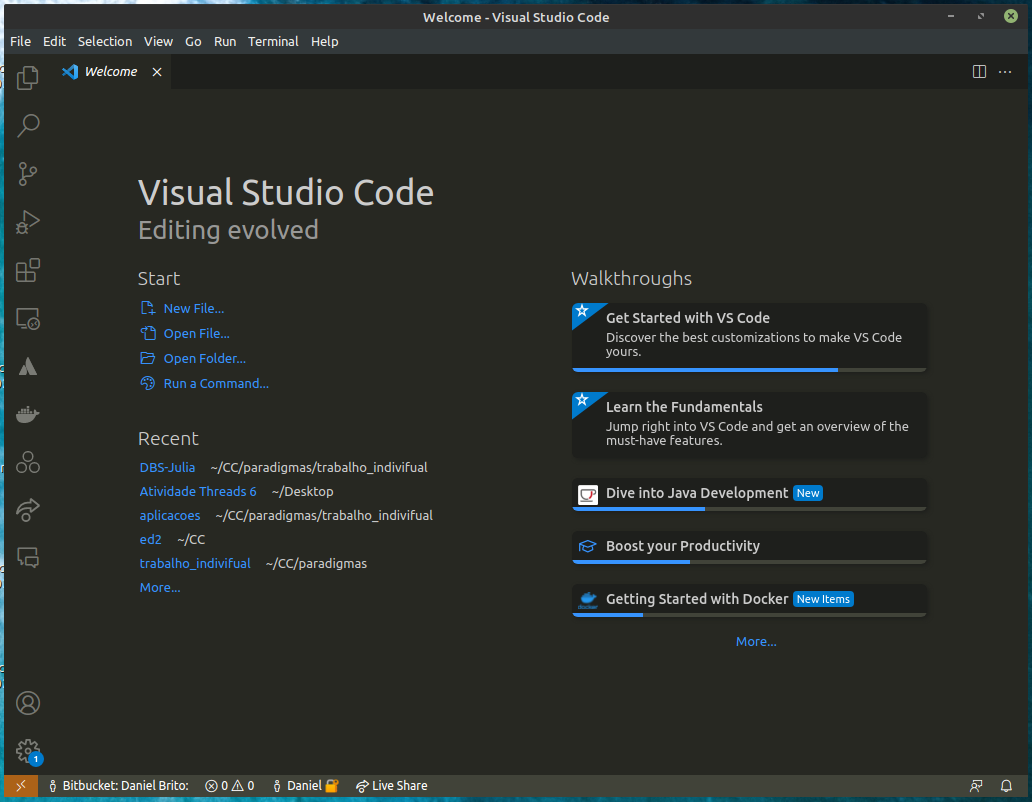
\includegraphics[width=12cm]{aplicacoes/VScode_welcome.png} \\
     {\tiny \sf Fonte: https://julialang.org/}
 \end{center}
\end{figure} 
Foi lançado em 2015\footnote{https://web.archive.org/web/20151009211114/http://blogs.msdn.com/b/vscode/archive/2015/04/29/announcing-visual-studio-code-preview.aspx}, e no mesmo ano seu código fonte foi publicado no GitHub com liçenca liberal MIT License. 
No ano seguinte figurou no 13º lugar das ferramentas mais utilizadas na pesquisa anual do Stack Overflow \footnote{https://insights.stackoverflow.com/survey/2021\#section-most-popular-technologies-integrated-development-environment}, mas logo ganhou popularidade de modo que desde 2018 tem sistematicamente mantido o primeiro lugar, e mesmo assim ganhando cada vez mais popularidade, nesse ano de 2021 ele foi citado por 70\% das respostas ao questionário. 

Dentro do ecossistema Julia percebemos um crescimento análogo, no qual o Vscode é atualmente utilizado por 62\% dos usuários da linguagem segundo a pesquisa de 2021. \footnote{https://julialang.org/blog/2021/08/julia-user-developer-survey}

O Visual Studio Code atualmente está na versão \href{https://github.com/microsoft/vscode/releases/tag/1.61.0}{1.61.0}, pode ser instalado por meio de seu site oficial \footnote{https://code.visualstudio.com/}.
\section{Jupyter Notebook}

O projeto Jupyter foi iniciado por Fernando Pérez e Brian Granger em 2015, a partir do projeto IPython também criado por Pérez. \footnote{https://bids.berkeley.edu/people/fernando-p\%C3\%A9rez}
O projeto se define como uma organização open-source sem fins lucrativos que busca desenvolver a ciência de dados e a computação científica interativas em todas as linguagens de programação, sempre de forma 100\% gratuita e livre. \footnote{https://jupyter.org/about}. 
%O IPython é um shell de comando interativo originalmente desenvolvido para python que permite uma série de funções desde interação, a computação paralela, flexibilidade, suporte a GUI e principalmente a interface que suporta código, texto, mídia, plots e expressões matemáticas, que foi a base na qual o Jupyter foi construído.

O nome Jupyter deriva das três linguagens que formam os pilares da computação científica -Julia, Python, R-. Também é uma homenagem aos cadernos astronômicos de Galileo, utilizados para registrar a descoberta das luas do planeta Júpiter. \footnote{https://blog.jupyter.org/i-python-you-r-we-julia-baf064ca1fb6}

Nesse contexto surge o Jupyter Notebook (Fig\ref{jupyter} ), um ambiente computacional baseado em web com cadernos interativos, copostos por células que podem conter código, texto, imagem, gráficos dentre outros. Um ambiente que promove a computação científica de diversas maneiras: em primeiro lugar pela experimentação que a independência de células permite ao executar separadamente partes de código, em segundo a documentação e reprodutibilidade nativas dos cadernos, que permitem registrar e compartilhar fluxos de trabalho e análise, além da integração com outras linguagens que podem por vezes ser necessárias dependendo das necessidados do projeto e o potencial de criar relatórios precisos e interativos nesse contexto. Motivo pelo qual a utilização de cadernos interativos se tornou o padrão em diversas áreas da técnologia da informação e ciências como por exemplo na ciência de dados e nas interface de Cloud como o Colaboratory do Google e o SageMaker da Amazon. \footnote{https://blog.jupyter.org/project-jupyter-computational-narratives-as-the-engine-of-collaborative-data-science-2b5fb94c3c58}

\begin{figure}[H]
\begin{center}
    \caption{Jupyter Notebook} \label{jupyter}
    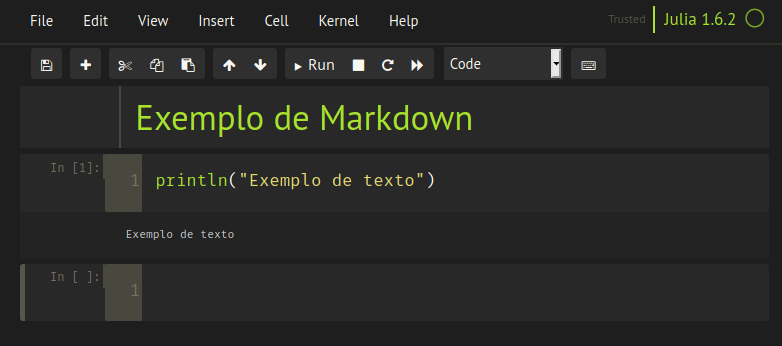
\includegraphics[width=12cm]{aplicacoes/jupyter.png} \\
    {\tiny \sf Fonte: Autor}
\end{center}
\end{figure} 


%The Jupyter Notebook has become a popular user interface for cloud computing, and major cloud providers have adopted the Jupyter Notebook or derivative tools as a frontend interface for cloud users. Examples include Amazon's SageMaker Notebooks,[26] Google's Colaboratory[27] and Microsoft's Azure Notebook.[28]

Para instalar o Jupyter Notebook, basta seguir as instruções disponíveis no site oficial do projeto \footnote{https://jupyter.org/install}, que atualmente se encontra na versão \href{https://github.com/jupyterlab/jupyterlab/releases/tag/v3.2.4}{3.2.4}.

\section{Pluto}
Assim como o Jupyter, Pluto apresenta cadernos interativos baseados em web. 
Sua principal diferença é ser escrito e executado puramente em Julia, sendo portanto mais leve. E também por ser reativo, isto é, cada mudança é automaticamente atualizada em todas as células afetadas, de modo que a qualquer momento o programa é completamente descrito pelo código apresentado. 

Pluto.jl foi criado por Fons Van der Plas e Mikołaj Bochenski, atualmente se encontra na versão 0.17.1 \footnote{https://github.com/fonsp/Pluto.jl\#readme}.  

Para utiliza-lo basta instalar o pacote no REPL Julia, e executá-lo conforme demonstramos na figura \ref{Pluto}. Já na figura \ref{Pluto_plot} apresentamos um dos cadernos de exemplo onde podemos ver sua estrutura, adequação ao texto e código. 

\begin{figure}[H]
\begin{center}
    \caption{Instalação e tela de boas vindas do Pluto.jl} \label{Pluto}
    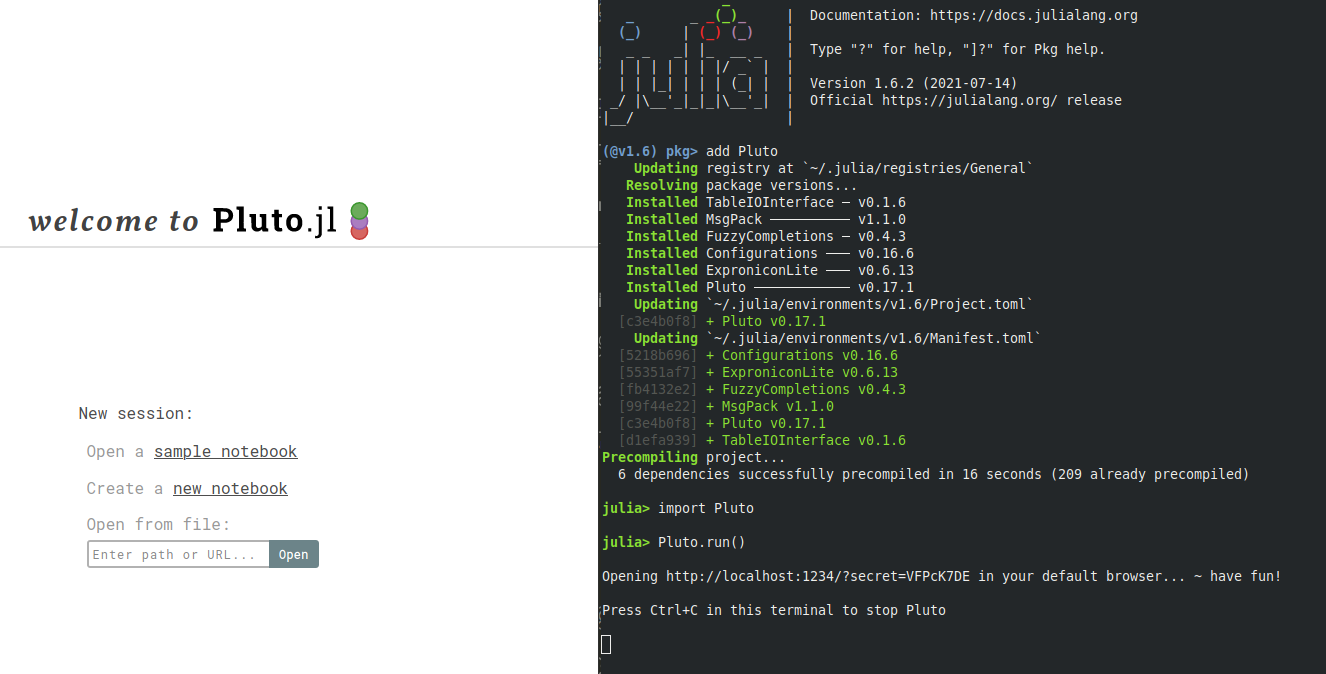
\includegraphics[width=12cm]{aplicacoes/Pluto.png} \\
    {\tiny \sf Fonte: Autor}
\end{center}
\end{figure} 

\begin{figure}[H]
\begin{center}
    \caption{Caderno de exemplo do Pluto.jl} \label{Pluto_plot}
    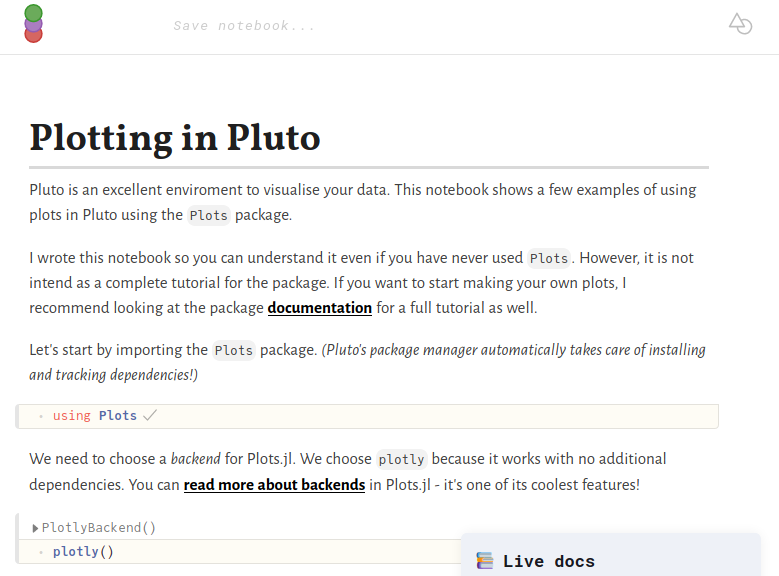
\includegraphics[width=12cm]{aplicacoes/Pluto_plotting.png} \\
    {\tiny \sf Fonte: Autor}
\end{center}
\end{figure} 